%qqqqqqqqqqqqqqqqqqqqqqqqqqqqqqqqqqqqqqqqqqqqqqqqqqqqqqqqqqqqqqqqqqqqqqqqq
%Quote
\begin{savequote}[50mm]
%‘‘El cosmos es todo lo que es, todo lo que fue y todo lo que será. Nuestras 
%más ligeras contemplaciones del cosmos nos hacen estremecer: Sentimos como 
%un cosquilleo nos llena los nervios, una voz muda, una ligera sensación como
%de un recuerdo lejano o como si cayéramos desde gran altura. Sabemos que nos
%aproximamos al más grande de los misterios.’’
%\qauthor{Carl Sagan}
\end{savequote}
%qqqqqqqqqqqqqqqqqqqqqqqqqqqqqqqqqqqqqqqqqqqqqqqqqqqqqqqqqqqqqqqqqqqqqqqqq




%#########################################################################
\chapter{Alineamiento de AGNs con su entorno a gran escala}
\label{cha:cosmic_web}

En esta sección se presentan los resultados obtenidos en la búsqueda de posible alineamiento del espín de los AGNs y el entorno cosmológico al cual pertenecen. Con al fin de poder llevar a cabo este propósito, se hace uso de: dos simulaciones cosmológicas ({\it{Cosmo01}} y {\it{Cosmo02}}), los los autovalores, autovectores, sobre densidades obtenidos con el método de T-Web y el catálogo FoF. A continuación se presentan las características de la simulaciones y de los resultados obtenidos.

%------------------------------------------------
\section{Características de las simulaciones}
\label{sec: propiedades en las simulaciones}
%------------------------------------------------

En la simulación hay parámetros o valores que dan información de la dinámica del sistema,  que arrojan criterios suficientes para decidir si lo obtenido está en acuerdo con los modelos físicos propuestos. 
Conforme a esto, se pretende realizar un análisis a la distribución de masa (función de masa) de los halos de materia, BHs y de estrellas. 

Debido a que no todos los halos hospedan un BH en su interior, fue necesario descartar los halos que no cumplen con esta condición. Esto reduce de gran manera la cantidad de galaxias a estudiar, sin embargo es suficiente para realizar un análisis adecuado.

%------------------------------------------------
\subsection{ Función de masa}
\label{subsec: funcion de masa}
%------------------------------------------------
La función de masa es uno de los parámetros de control más contundentes en el análisis de las simulaciones. Bajo la teoría de formación y evolución de galaxias se tiene que los objetos con baja masa son más abundantes, debido a que en los procesos evolutivos de las galaxias la interacción es jerárquica, las galaxias más masivas tiene una mayor probabilidad en fusionarse con otras debido a su gran potencial gravitacional, esto hace que las galaxias más densas se terminen fusionando y disminuyendo su población. Con base a esto la función de masa de las galaxias (halos, BHs y masa estelar) debe decrecer a medida que se aumentan las masas, i.e., La cantidad de objetos disminuye a medida que aumenta la masa, es menos probable encontrar BHs muy masivos. 
%
\begin{figure}[-h]
 \centering
  \subfloat{
   \label{fig: función de masa BHs}
    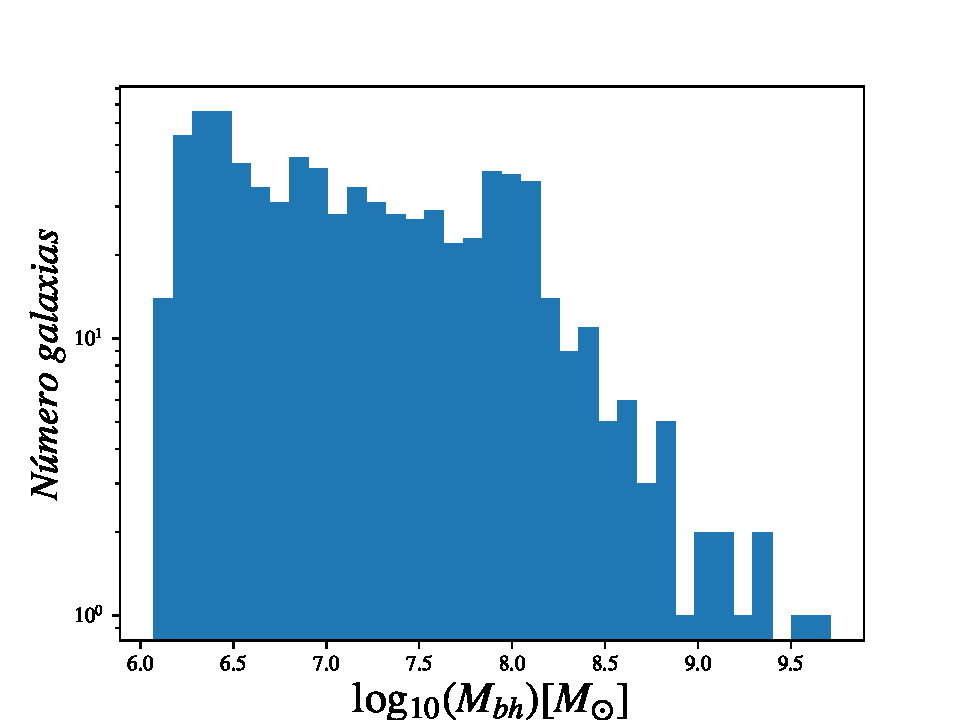
\includegraphics[width=0.32\textwidth]{./figures/6_Resultados/cosmo01/histo_Mass_bh.pdf}}
  \subfloat{
   \label{fig: función de masa halos}
    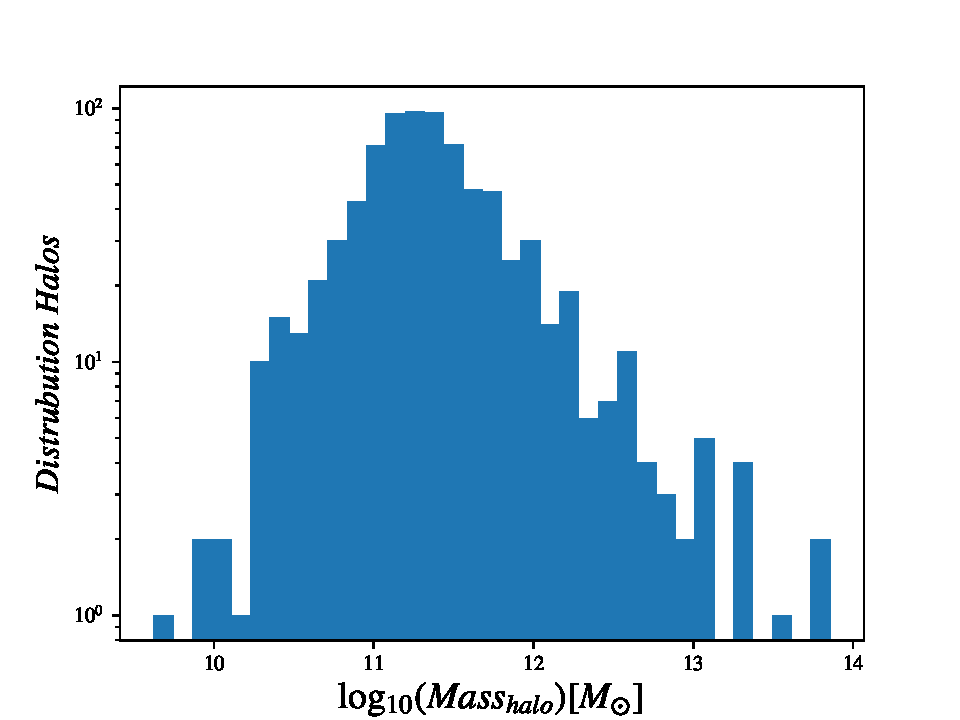
\includegraphics[width=0.32\textwidth]{./figures/6_Resultados/cosmo01/histo_Mass_halos.pdf}}
  \subfloat{
   \label{fig: función de masa estelar}
    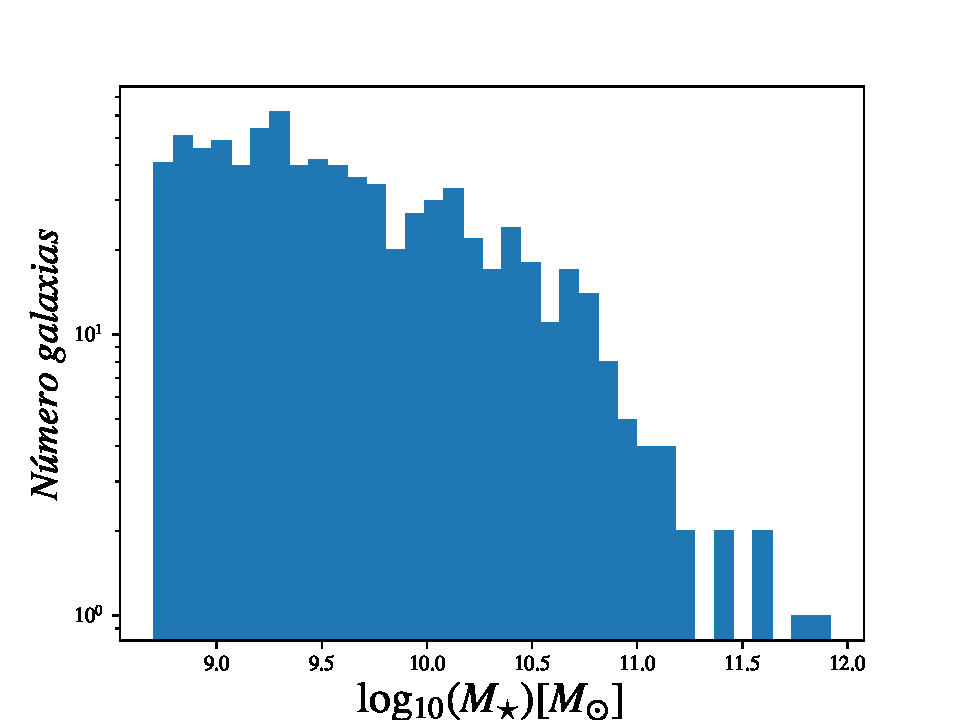
\includegraphics[width=0.32\textwidth]{./figures/6_Resultados/cosmo01/histo_Mass_stelar.pdf}}
 \caption{Funciones de masa para agujeros negros, halos y masa estelar, estas información da cuenta del número de objetos con una masa determinada, esto se realizo para {\it{Cosmo01}}. }
 \label{fig: Funciones de masa cosmo01}
\end{figure}
 %%%%%%%%%%%%%%%%%%%%%%%%%%%%%%%%%%%%%%%%%%%
 \begin{figure}
 \centering
  \subfloat{
   \label{fig: función de masa BHs}
    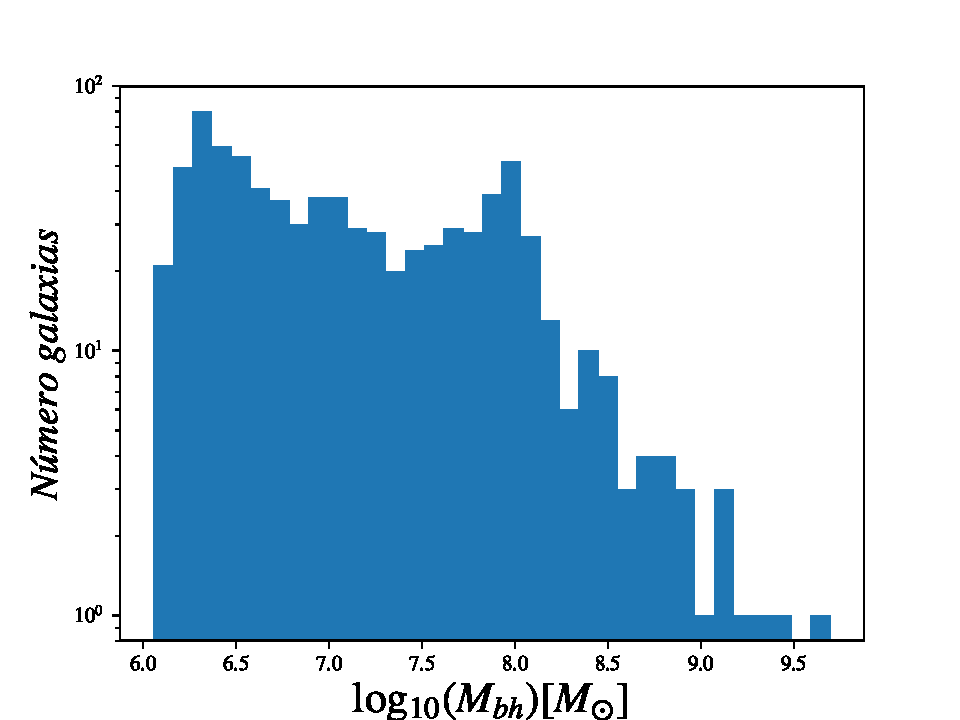
\includegraphics[width=0.32\textwidth]{./figures/6_Resultados/cosmo02/histo_Mass_bh.pdf}}
  \subfloat{
   \label{fig: función de masa halos}
    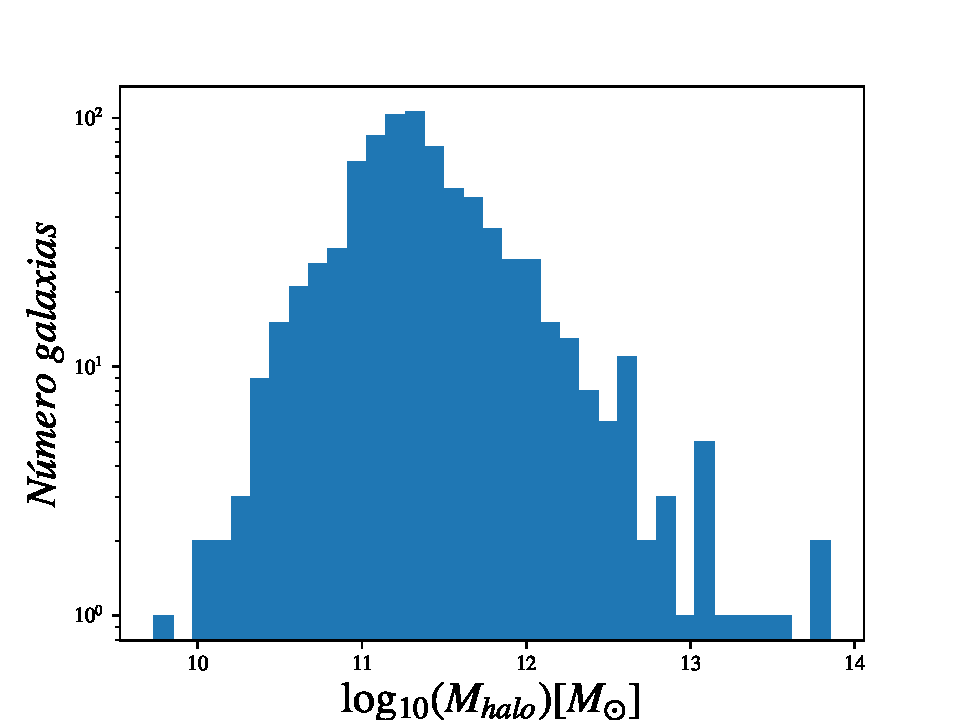
\includegraphics[width=0.32\textwidth]{./figures/6_Resultados/cosmo02/histo_Mass_halos.pdf}}
  \subfloat{
   \label{fig: función de masa estelar}
    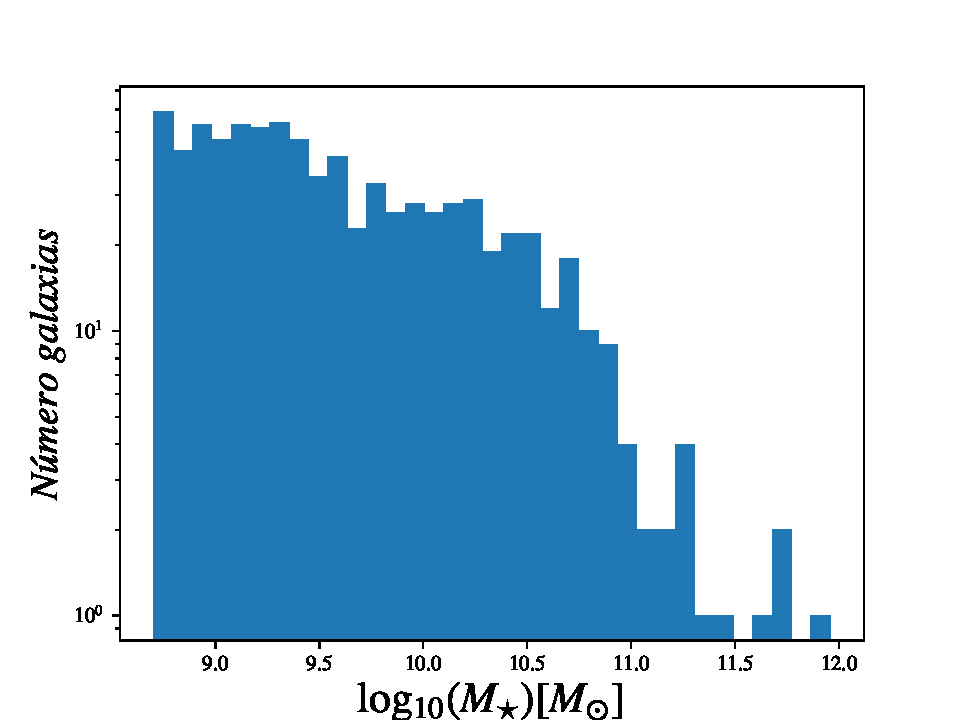
\includegraphics[width=0.32\textwidth]{./figures/6_Resultados/cosmo02/histo_Mass_stelar.pdf}}
 \caption{Funciones de masa para agujeros negros, halos y masa estelar, estas información da cuenta del número de objetos con una masa determinada, esto se realizo para {\it{Cosmo02}}.}
 \label{fig: Funciones de masa cosmo02}
\end{figure}
%
Al observar las figuras (\ref{fig: Funciones de masa cosmo01} y \ref{fig: Funciones de masa cosmo02}), es posible concluir que los resultados de la simulación son congruentes con la teoría y con las observaciones. Para despreciar los posibles errores producto de la baja resolución en galaxias de baja masa, se consideran sistemas en los cuales las masa estelar sea mayor a $5\times 10^{8}M_{\odot}$. Este criterio hace que la distribución de masa para los halos presente  esa extraña forma, con esta gráfica es posible argumentar que los halos de baja masa presentan una gran numero de masa estelar menor a $5\times 10^{8}M_{\odot}$, a medida que aumenta la masa del halo el numero de objetos con masa estelar menos al criterio disminuye. 

A parte de la función de distribución de masa es posible usar otros criterios que den información de la simulación y de su veracidad. 

La teoría sobre la formación de galaxias indica la existencia de una relación lineal entre la masa estelar de una galaxia y del BH anfitrión, por tanto las galaxias que poseen una masa estelar considerable poseen un BH con una masa considerable también. Por tanto las simulaciones debe reproducir este resultado teórico y observacional. Al observa las figuras (\ref{fig: Mass_bhVsMass_stelar}), es posible observar que las simulaciones bajo este criterio, también reproducen las observaciones. 
%
 \begin{figure}[-h]
 \centering
  \subfloat{
   %\label{fig: mass_bhVsmass_stelar}
    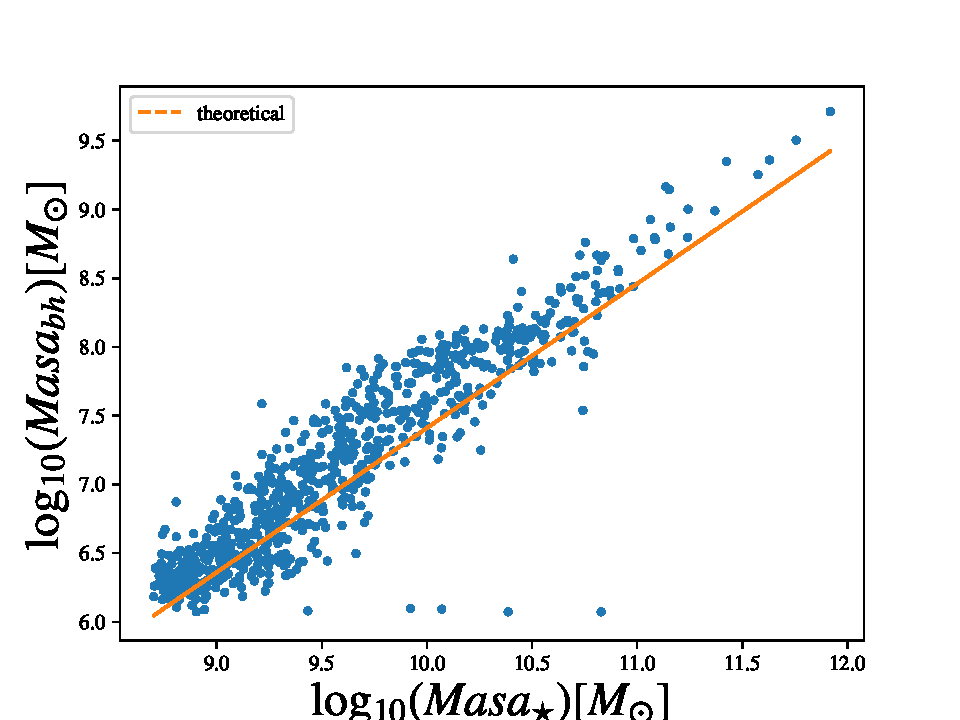
\includegraphics[width=0.49\textwidth]{./figures/6_Resultados/cosmo01/Mass_bhVsMass_stelar_halo.pdf}}
  \subfloat{
   %\label{fig: función de masa halos}
    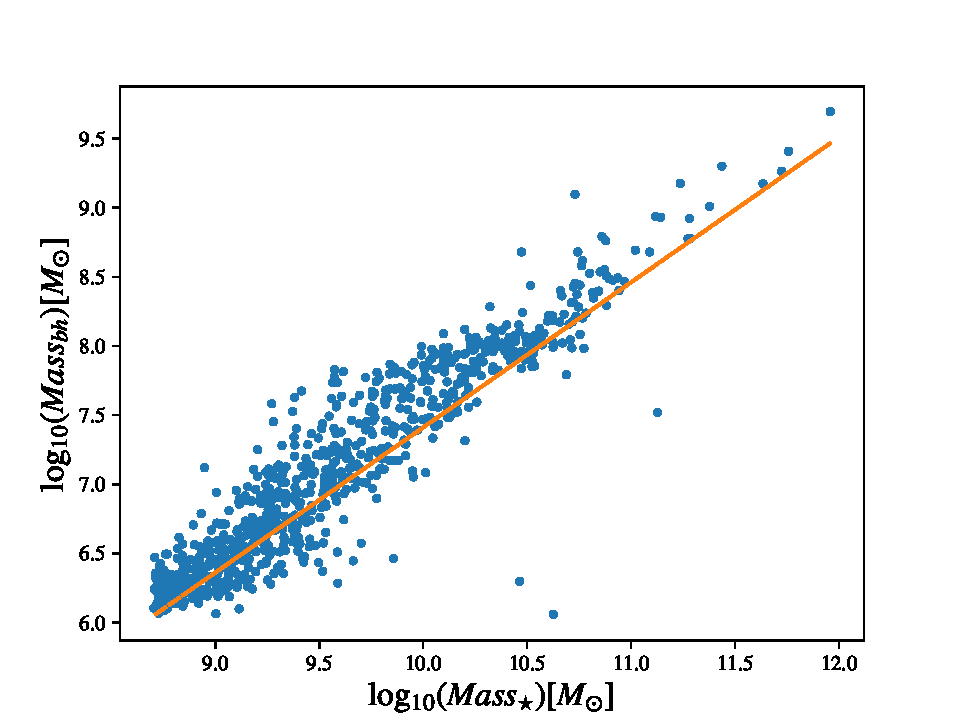
\includegraphics[width=0.49\textwidth]{./figures/6_Resultados/cosmo02/Mass_bhVsMass_stelar_halo.pdf}}
 \caption{Relación Masa BH y Masa estelar, según los resultados observacionales hay una dependencia lineal entre la masa del BH y la masa estelar para cada galaxia. La imágen de la derecha pertenece a {\it{cosmo01}} y el de la izquierda a {\it{cosmo02}}. La linea naranjada es la teórica\cite{McConnell2013}, con la cual se puede asegurar que la simulación es consistente con lo observacional.}
 \label{fig: Mass_bhVsMass_stelar}
\end{figure}
%
%------------------------------------------------
\subsection{ Distribución de galaxias en el entorno cosmológico}
\label{subsec: Distribucion de galaxias}
%------------------------------------------------

La distribución de las galaxias en el entorno cosmológico son determinantes en el resultado de final de este trabajo. Es necesario entonces poder concluir que los resultados obtenidos por las simulaciones reproduzcan las observaciones. Haciendo uso de método de T-Web, se extraen los autovalores $\lambda_{i}$, los autovectores $\vec{e}_{i}$ y la sobre densidad $\delta$. 

Como se explico en la sección (\ref{subsec: Metodo_T-web}),  los autovalores son los responsables de clasificar los entornos y con ello a las galaxias. Es necesario contrastar que la distribución de galaxias debe ser equivalente al mapa de sobre densidades. 

Al observar las distribución de BHs en el espacio, se observa que gran parte de los BHs se ubica en los cluster o filamentos. Este resultado puede ser contrastado con el valores de los autovalores $\lambda_{i}$, al observar la figura (... ) también se puede concluir lo siguiente:  $\lambda_{1}\geq 0$,  $\lambda_{2}\geq 0$ y $\lambda_{3}$ esta acotado entre $-10 \leq \lambda_{3}\leq 10$, mayormente con valores positivos.



%***********************************************************************